\begin{tikzpicture}
    \pgfmathsetmacro{\a}{0}
    \pgfmathsetmacro{\b}{5.5}
    \pgfmathsetmacro{\c}{7}

    \draw [ultra thick] (\a, 0) -- (\c, 0);
    \foreach \x in {\a, \b, \c} {
        \draw (\x, 0.2) -- (\x, -0.2);
    }
    \draw[decorate, decoration={brace, amplitude=0.3cm}] (\a, 0.3) -- (\c, 0.3)
        node [pos=0.5, above=1em, align=center] {$14x$};
    \draw[decorate, decoration={brace,mirror, amplitude=0.3cm}] (\a, -0.3) -- (\b, -0.3)
        node [pos=0.5, below=1em, align=center] {$5 \times \dfrac{3}{10}$};
    \draw[decorate, decoration={brace,mirror, amplitude=0.3cm}] (\b, -0.3) -- (\c, -0.3)
        node [pos=0.5, below=1em, align=center] {$5x$};
\end{tikzpicture}
